\chapter{Declarative vs. imperative systems} \label{imperative}

Different approaches to declarative modeling of
systems design are presented. Endres et al. \cite{endres2017declarative} compare declarative and imperative
standpoints in a cloud computing context and collect systematic
information on what are the strengths and weaknesses of TOSCA, IBM
Bluemix, Chef, Juju, and OpenTOSCA. Van
der Burg and Eelco Dolstra \cite{van2010declarative} use NixOS as a solution for declaratively
distributing into cloud, executing integration and system tests. Most approaches researched through
literature review focus on distributing to cloud. Distributing to
embedded clearly remains a niche.

Breitenbücher et al. \cite{breitenbucher2017declarative} focus on deploying into embedded and discuss
the challenges an IoT user face when deploying a system. It is proven
that setting up devices with mandatory scripts and other actions is a
challenging task, when a number of devices should be set up \cite{breitenbucher2017declarative}. Cloud is
something that is practical to be used in tandem with IoT, but this thesis
focuses on an \textit{in-premises} reference
solution. 

In this chapter, we focus on comparing different declarative
approaches to the more traditional imperative models, highlighting the
strengths and weaknesses of both. Specifically, examples are provided
to illustrate the limitations often observed in imperative systems,
particularly in terms of reproducibility, scalability and
administration standpoints. Cloud-oriented approaches serve as a key
reference point for the effective distribution and automation of
declarative systems. It can be argued that similiar approaches as
those taken in cloud, should be taken in embedded and IoT to increase
security through updatability and upgradability. This argument is backed up
in section \ref{improvingwithnix}, where a concrete use case is demonstrated.

\section{Imperative systems}

Imperative deployment models base their functionalities through a
process in which the order of events have a critical significance to
the output \cite{breitenbucher2017declarative}. In the context of
virtualisation, imperative tooling can be used to form all
activities to be executed: the control flow, execution order
and the data flow between them \cite{endres2017declarative}. This kind
of process is best to be used in conjunction with a formalised
workflow or standard such as BPEL \cite{endres2017declarative}. In
contrast, declarative models don't have such specific requirements, as
these models formalise the processes in the configuration files
\cite{endres2017declarative}.

Imperative systems have inherent problems regarding
administrative traits contributing to a framework where the underlying
system has \textbf{no traceability}: the implication that
reproducibility is impossible, as changes to a system are not
traced. Nix provides a solution for this problem with its Nix
generation system \cite{dolstra2007purely}. With
imperative systems, upgrading is more error-prone than installing from
scratch. This is due to the fact that imperative systems have
\textbf{unpredictable} state, from where the system should migrate to
a predictable state. This causes major issues regarding
upgradability. 

\textbf{The inability to run multiple configurations side-by-side} is
an inherent side effect of a \textit{stateful} system \cite{dolstra2007purely}. Declarative
systems don't have this problem: an arbitrary number of configurations
can exist side by side, as the system is defined only by the
configuration, not with the state as a
component. 

\subsection{Debian/Apt} \label{debian/apt}

An example of imperative systems' problematic nature is provided with
the following demonstration. Executing shell command
\begin{lstlisting}
    apt install emacs
\end{lstlisting}
installs a text editor wrapped as a .deb package.  The package emacs
has a dependency, emacs-gtk, which can be removed with command
\begin{lstlisting}
    apt remove emacs-gtk
\end{lstlisting}
Another dependency, emacs-lucid can be removed with command
\begin{lstlisting}
    apt remove emacs-lucid
\end{lstlisting}

we can see that after removing, apt automatically installs emacs-gtk
to avoid breaking the application. The package manager warns:
''emacs-lucid has dependency problems, but removing anyway as you
requested'' as shown in figure \ref{deb_remove}. It is also noteworthy,
that the manual page for apt does not tell anything about a possible
installation side-effect of a package removal command
\cite{ubuntuUbuntuManpage}. We could forcibly remove the package by
invoking
\begin{figure}[H]\label{dpkgsnippet}
\begin{lstlisting} 
    dpkg --remove --force-depends emacs-lucid
\end{lstlisting}
\end{figure}
% kuva distribuutioiden distribuutioista
\begin{figure}[b]\label{deb_remove}
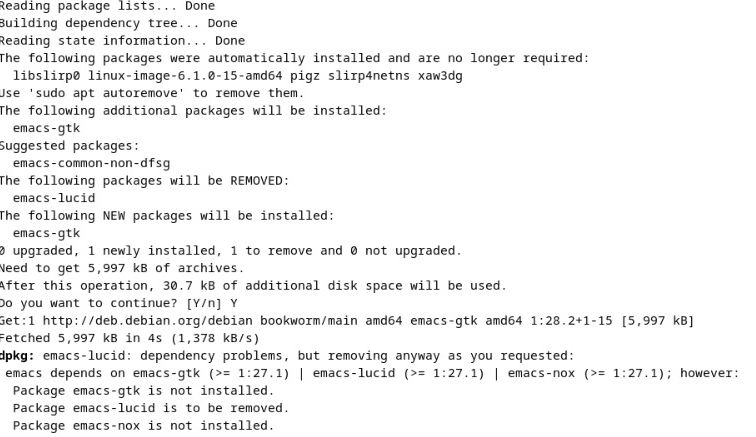
\includegraphics[scale=2.0]{latex/kuvat/cropped_apt_output.jpg}
\caption[Terminal output from Emacs installation.]{Terminal output from a Debian system when installing an Emacs package.}
\end{figure}
leaving the system in an unreliable state. Dpkg is a low-level
tool associated with apt, which does not automatically handle dependency
resolutions or further package relations
\cite{thiruvathukal2004gentoo}. What happens if we had a large number
of devices, in-premises or cloud, where all system commands are done
imperatively? We would have a large number of devices that differ from
each other, because as shown, the order of commands affect the state
of the system. Time is also a factor that
causes systems to diverge as packages are not up-to-date by
default. Invoking 
\begin{figure}[H]\label{aptupdate}
\begin{lstlisting} 
  apt update
\end{lstlisting}
\end{figure}
updates the local repositories to match the download mirrors. If by
technical reasons or possible user error the commands are conducted in
the wrong order, this will lead to divergent systems.

Implementing a deployment model with only Debian would be a gruesome
task as the order of events, which occur during the setup phase, is
critical. As presented by Endres et al. \cite{endres2017declarative} a formalised workflow graph
would be needed to set up a reliable system. However, Debian could
be used as a host to user-space application deployment such as
Bluemix or Chef, where common DevOps practices can be used.

\section{Declarative systems} \label{declarativesystems}

Presented problems in section \ref{debian/apt} can be solved using a
reproducible, reliable and atomic package manager. In Nix, package
installations are isolated from one another to prevent conflicts,
ensuring they function consistently even if the underlying
installations differ. As packages are declared in a single set of
configuration files, it is trivial to reproduce the system in a
different environment. The demonstrated effect in snippet
\ref{dpkgsnippet} was a problem due to lack of isolation. When
dependencies are scattered in the system instead of declared
explicitly in an installed package, a faulty state could be
achieved. Nix assures, that these kinds of problems are out of the
question. A result of this is that in a Nix system installs of same
program can reside side-by-side with varying versions
\cite{dolstra2008nixos}.

As presented by Endres et al. \cite{endres2017declarative} systems can be declared, even if the
underlying infrastructure is imperative by nature. This thesis focuses on purely functional
methodologies which fix the most prevalent issues found in
imperative models. Tools such as Chef focus on deploying on an
imperative system, which causes an inherent problem with cohesion in a
system that should work regardless of the underlying machine or
network. Alternative deployment tools are discussed in section
\ref{nondeclarative}.

One benefit from Nix is its lightweight option to enable system
tests. Integrating system tests with a Debian system would require a
considerable amount of work, as setting up such system needs a lot of
configuration and executing commands in a correct order
\cite{van2010automating}. Debian definitely fits in an imperative
deployment strategy but the requirement for explicit detail of every
step would be prone to errors even for a seasoned administrator
\cite{breitenbucher2017declarative}.

It is also noteworthy that many imperative package managers do not 
support rollback mechanisms. If the Nix configuration file is changed
and the system is rebuilt with command
\begin{lstlisting}
nixos-rebuild switch
\end{lstlisting}
the previous state could be recovered by
\begin{lstlisting}
nix profile rollback
\end{lstlisting}
This is an important feature since the Nix configuration files control
the whole system, they can also leave the system in an undesired
state. Nix switches between \textit{profiles}, which is a way to
provide different configurations for different user environments as
shown in figure \ref{userenvs}, providing atomic upgrades and
rollbacks \cite{nixosNixOSManual}.

A fundamental component of the ecosystem is Nix, a domain-specific
language designed for configurations, distinguished by its functional
nature and lazy evaluation. The concept of purity is central to Nix,
where values remain unchanged throughout computation and every
function consistently yields the same output regardless of input
\cite{dolstra2013charon}. The security implications of using Nix
vs. an imperative system are discussed in the next chapter.

\subsection{Non-declarative components} \label{nondeclarative}

Declarative distributions such as Nix cannot do everything in the
system in stateless manner. Some components of the system such as
databases must have a distinct state, which cannot be practically
declared with package manager apart from initial configurations
\cite{van2013reference}. Home directories can vary as much as the
system administrator desires. For example, a configuration file for
text editor vim is usually declared in the file
\begin{lstlisting}
  /home/<user>/.vimrc.
\end{lstlisting}
Nix provides multiple ways to perform the whole
configuration process from the Nix configuration files. One way is
declaring the desired .vimrc in the Nix configuration, as in the
following program snippet:

\begin{lstlisting}
{
  environment.systemPackages = [
    (pkgs.vimConfigurable.customize {
      vimrcConfig.customRC = ''
        " arbitrary vim config
      '';
    })
  ];
}
\end{lstlisting}
Nix also provides ways to fetch content to the system from
remote URLs. If the administrator does not want the system to
remain ''pure'', they can also build the system by
\begin{lstlisting}
  nixos-rebuild switch --impure
\end{lstlisting}
This results in the system having mutable components, which can be
desirable from an accessibility point of view, but can cause
unpredictable behaviour if the impure components are modified. Purity means that the components are read-only and
immutable \cite{dolstra2010nixos}.

User environments (Nix profiles) can be used in multiple environments for different users, in which the user can operate as shown in figure  \ref{userenvs}. User
environments are a successor to the concept, where installed programs
either reside in
\begin{lstlisting}
/usr/bin
\end{lstlisting}
or
\begin{lstlisting}
/usr/sbin
\end{lstlisting}
or have a symbolic link to
the said directories. They can be figured as trees of symbolic links
that reside also in the Nix store hence referred packages are called
''activated packages'' \cite{dolstra2008nixos}. The installed programs reside usually in
\begin{lstlisting}
  /nix/store
\end{lstlisting}

\begin{figure}[t!]
\centerline{\includesvg[width=1.0\columnwidth]{latex/kuvat/symlinks.drawio.svg}}
\caption[Relation graph in Nix environment.]{Relations between different user environments and installed
  programs \cite{nixosUserEnvironment}.}
\label{userenvs}
\end{figure}

Continuous build and integration services such as Hydra,
which include Nix-compatible support for handling runtime
configuration and tools such as Disnix and Charon\footnote{Charon is
now called NixOps \cite{githubNixNixpkgsNixOS}}, focus on
setting up complementary infrastructure. Van Der Burg \cite{van2013reference} presents these
new tools to replace Cfengine, Puppet and Chef, which execute
operations in convergent manner, meaning that they capture what
changes should be done to the machines in a specified
network.

These approaches have two central problems: imperative nature of
handling environment difference and inability to guarantee
configuration compatibility with a machine. Disnix is a Nix derivative
that can overcome these challenges by separating logical properties
from physical and capturing the essential aspects which form a
system \cite{van2013reference}.

\subsection{Home manager and flakes}

Nix environments can be built from a single configuration.nix file,
but there are two significant configuration tools for managing Nix
systems: home manager and flakes. Home manager is an extension for
managing user profiles with a declarative Nix syntax
\cite{nixcommunityHomeManager}. However home manager has issues with atomic
rollbacks and for this reason they are not used in this thesis'
examples.

Flakes is an experimental feature of Nix, which provides environments, where
dependencies are pinned in a lock file, further improving
reproducibility of Nix systems \cite{nixosFlakesNixOS}. A flake is a
file system tree which contains a root directory with the Nix lock file
specification called flake.nix. The usage of flakes is a favorable method
for organising different environments within a Nix system where it
can consist of multiple flakes. Flakes is an experimental
feature, thus out of this thesis' scope. 

\subsection{Ease of updates}

Due to atomic rollbacks, updating with Nix is easy and riskless. Nix
handles software providing through channels. A channel is a set of
latest Git commits in a Nixpkgs repository, where they are divided to
stable/unstable and large/small channels
\cite{nixosChannelsNixOS}. Unstable channels (large and small) have
the latest commits on a rolling basis, but include less conservatively
checked functionalities. Stable channels are submitted through a
version number (e.g. 23.11), where a new release is published every
six months. Large channels contain a full set of Nixpkgs binaries,
when small ones include a subset. If a system administrator decides to
submit to a small channel, they have more recent updates at their
disposal, but have to resort to compiling some needed packages from
source.

Updating a Nix system is just a manner of invoking command

\begin{lstlisting}
sudo nix-channel --update
\end{lstlisting}
and if stable release is chosen, changing the
\begin{lstlisting}
system.stateVersion
\end{lstlisting}
from the configuration.nix file \cite{nixosNixOSManual}. Nixpkgs is a
repository of working Nix packages using a continuous integration
service called Hydra. Hydra evaluates the needed Nix expression of a
package and ensures its functionality \cite{nixosNixOSManual}.

It is apparent that purely functional and declarative approaches are not as popular
as imperative systems due to the need of steep learning curves and
obscure syntax. This can be seen as historical payload: imperative
models have been in use a longer time than purely functional
approaches such as Nix.

In this chapter we revealed, that declarative systems have inherent
strengths in both deployment strategies and system upgrading. The next
section brings up the security viewpoint of declarative systems
specifically in an embedded Linux setting.
